\documentclass[tikz,border=14pt]{standalone}
\usepackage{amsmath,amssymb}
\usetikzlibrary{arrows.meta}
\definecolor{ink}{HTML}{E4EDF8}
\definecolor{muted}{HTML}{596B80}
\definecolor{blue}{HTML}{9FC2FF}
\definecolor{teal}{HTML}{63D3BB}
\definecolor{gold}{HTML}{E7C274}
\definecolor{panel}{HTML}{111923}
\pagecolor{panel}
\color{ink}
\begin{document}
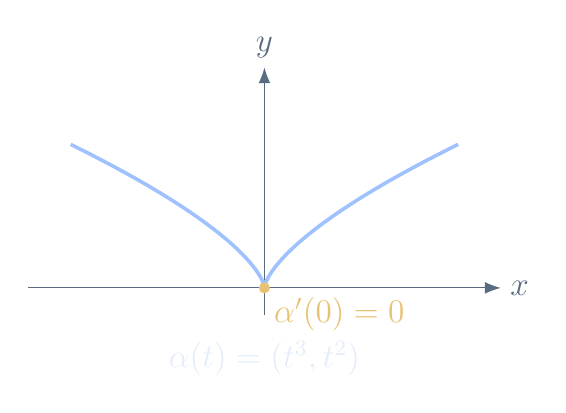
\begin{tikzpicture}[font=\large,text=ink,vec/.style={-{Latex[length=3mm]},line width=1.3pt},axis/.style={muted,-{Latex[length=2mm]},thin}]

\draw[axis] (-3,0)--(3,0) node[right] {$x$};\draw[axis] (0,-.35)--(0,2.8) node[above] {$y$};
\draw[blue,line width=1.3pt] plot[domain=-1.35:1.35,samples=140] ({\x*\x*\x},{\x*\x});
\fill[gold] (0,0) circle(2pt) node[below right] {$\alpha'(0)=0$};
\node[text=ink] at (0,-.9) {$\alpha(t)=(t^3,t^2)$};

\end{tikzpicture}
\end{document}
